\documentclass[aspectratio=169]{beamer}

\usetheme{default}
\setbeamertemplate{navigation symbols}{}
\setbeamertemplate{enumerate item}{\color{navy}\arabic{enumi}.}
\setbeamertemplate{itemize item}{\color{black}\textbullet}
\setbeamertemplate{itemize subitem}{\color{black}\textbullet}
\usepackage{booktabs}
\usepackage{xcolor}
\usepackage{tikz}
\usetikzlibrary{shapes,arrows,positioning}
\definecolor{navy}{RGB}{0, 0, 128}
\definecolor{lightblue}{RGB}{230,240,250}
\definecolor{darkgreen}{RGB}{0,100,0}
\definecolor{lightgreen}{RGB}{230,250,230}
\newcommand{\highlight}[1]{\colorbox{lightblue}{$\displaystyle\textcolor{navy}{#1}$}}
\newcommand{\highlighttext}[1]{\colorbox{lightblue}{\textcolor{navy}{#1}}}
\newcommand{\highlightgreen}[1]{\colorbox{lightgreen}{$\displaystyle\textcolor{darkgreen}{#1}$}}

\usepackage{hyperref}
\hypersetup{
    colorlinks=true,
    linkcolor=navy,
    urlcolor=navy,
    citecolor=navy
}

\begin{document}

\begin{frame}

Why is learning important in economics?

\bigskip{}

\begin{itemize}
\itemsep1.5em
\item<2-> Uncertainty and learning can explain some empirical puzzles
\bigskip\par
    \begin{itemize}
    \item<3-> Why engage in something costly and not finish it? (e.g. college)
    \end{itemize}
\item<4-> Agents might act differently if they had greater amounts of information
\item<5-> This means we need to model how \textit{beliefs} map into \textit{actions}
\bigskip\par
    \begin{itemize}
    \item<6-> $\implies$ learning should be part of a DDC model!
    \end{itemize}
\item<7-> A persistent question is how can we help agents become more informed?
\item<8-> Information is valuable, but usually costly to obtain
\end{itemize}

\end{frame}










\begin{frame}
Education papers that use learning models:
\bigskip\par
\begin{itemize}
\itemsep1.5em
\item High school dropout (Fu et al. 2022 QE)
\end{itemize}
\end{frame}

\begin{frame}
\centering
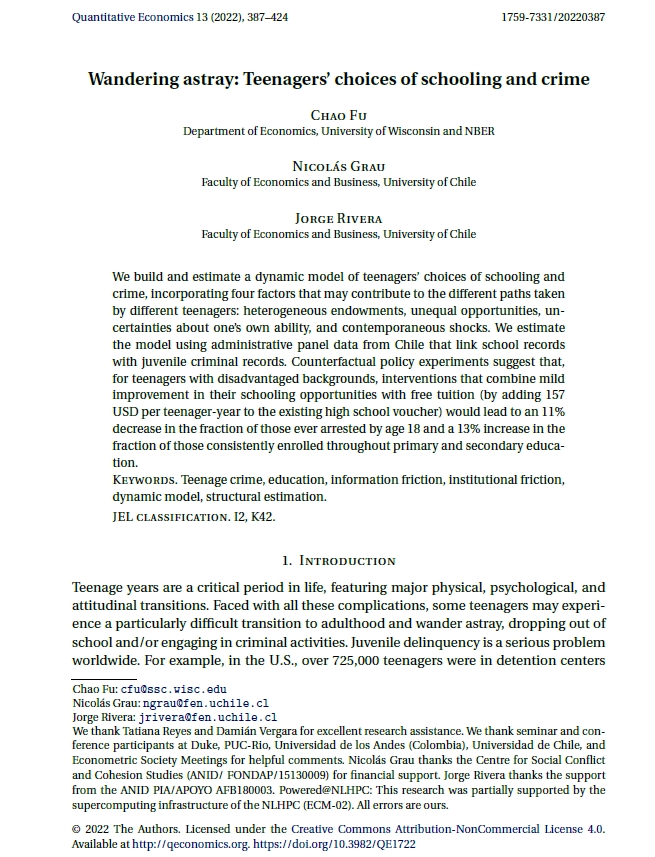
\includegraphics[width=0.45\textwidth]{Fu_al_cover.jpg}
\end{frame}


\begin{frame}
Education papers that use learning models:
\bigskip\par
\begin{itemize}
\itemsep1.5em
\item High school dropout (Fu et al. 2022 QE)
\item College major choice (Arcidiacono 2004 JE)
\end{itemize}
\end{frame}

\begin{frame}
\centering
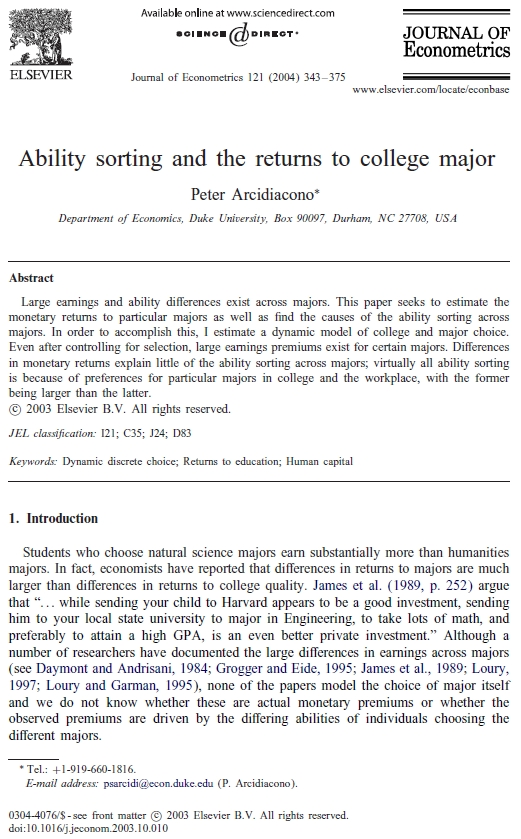
\includegraphics[width=0.36\textwidth]{Arcidiacono_2004_JE_cover.jpg}
\end{frame}


\begin{frame}
Education papers that use learning models:
\bigskip\par
\begin{itemize}
\itemsep1.5em
\item High school dropout (Fu et al. 2022 QE)
\item College major choice (Arcidiacono 2004 JE; Stinebrickner \& Stinebrickner 2014 REStud)
\end{itemize}
\end{frame}

\begin{frame}
\centering
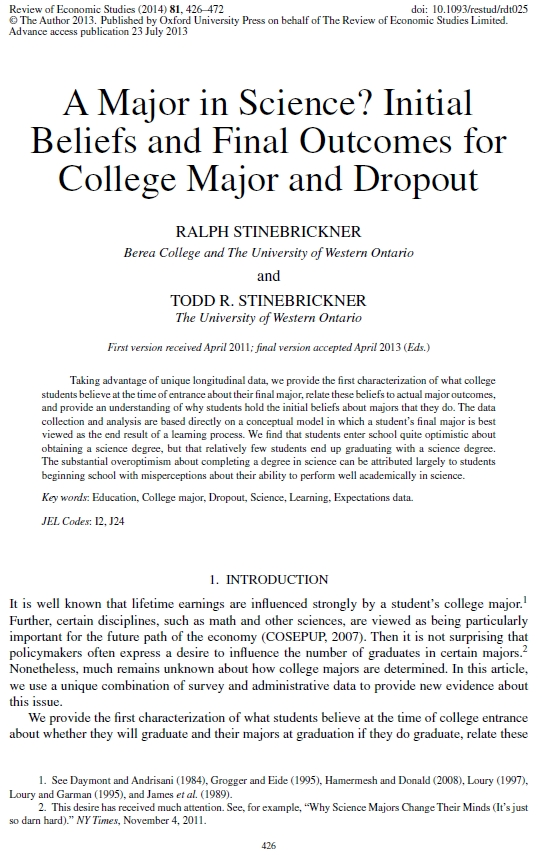
\includegraphics[width=0.36\textwidth]{Stinebrickner2_2014_REStud_cover.jpg}
\end{frame}


\begin{frame}
Education papers that use learning models:
\bigskip\par
\begin{itemize}
\itemsep1.5em
\item High school dropout (Fu et al. 2022 QE)
\item College major choice (Arcidiacono 2004 JE; Stinebrickner \& Stinebrickner 2014 REStud)
\item College dropout (Stinebrickner \& Stinebrickner 2014 JOLE)
\end{itemize}
\end{frame}

\begin{frame}
\centering
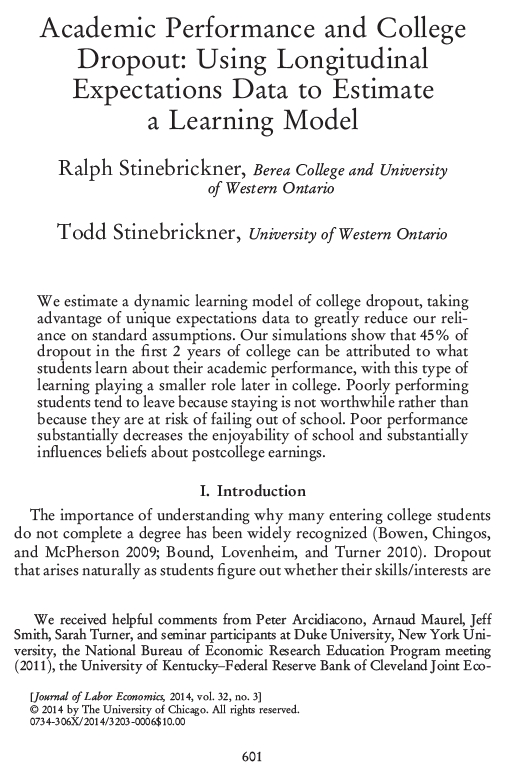
\includegraphics[width=0.4\textwidth]{Stinebrickner2_2014_JOLE_cover.jpg}
\end{frame}


\begin{frame}
Education papers that use learning models:
\bigskip\par
\begin{itemize}
\itemsep1.5em
\item High school dropout (Fu et al. 2022 QE)
\item College major choice (Arcidiacono 2004 JE; Stinebrickner \& Stinebrickner 2014 REStud)
\item College dropout (Stinebrickner \& Stinebrickner 2014 JOLE; Arcidiacono et al. 2025 JPE)
\end{itemize}
\end{frame}

\begin{frame}
\centering
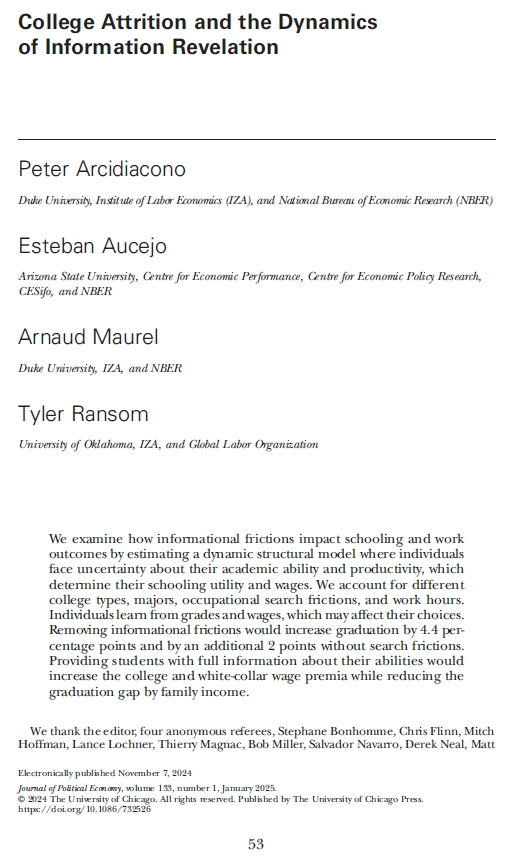
\includegraphics[width=0.36\textwidth]{AHMR_2025_JPE_cover.jpg}
\end{frame}








\begin{frame}
Labor papers that use learning models:
\bigskip\par
\begin{itemize}
\itemsep1.5em
\item Occupational choice (Miller 1984 JPE)
\end{itemize}
\end{frame}

\begin{frame}
\centering
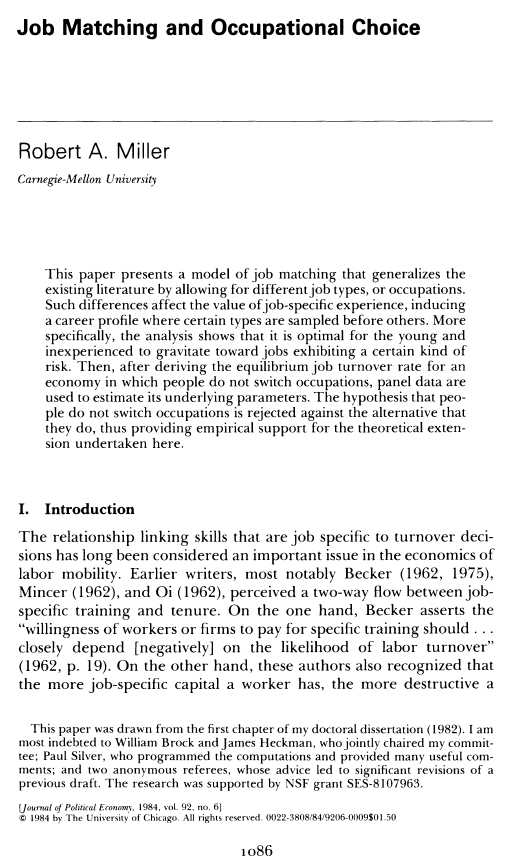
\includegraphics[width=0.36\textwidth]{Miller_1984_JPE_cover.jpg}
\end{frame}


\begin{frame}
Labor papers that use learning models:
\bigskip\par
\begin{itemize}
\itemsep1.5em
\item Occupational choice (Miller 1984 JPE)
\item Employee quality (Farber \& Gibbons 1996 QJE)
\end{itemize}
\end{frame}

\begin{frame}
\centering
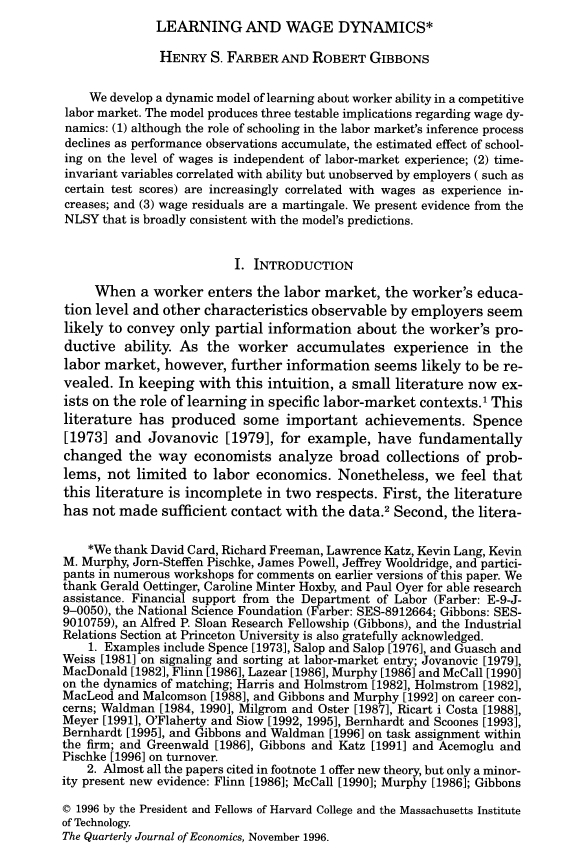
\includegraphics[width=0.44\textwidth]{Farber_Gibbons_1996_QJE_cover.jpg}
\end{frame}

\begin{frame}
Labor papers that use learning models:
\bigskip\par
\begin{itemize}
\itemsep1.5em
\item Occupational choice (Miller 1984 JPE)
\item Employee quality (Farber \& Gibbons 1996 QJE; Altonji \& Pierret 2001 QJE)
\end{itemize}
\end{frame}

\begin{frame}
\centering
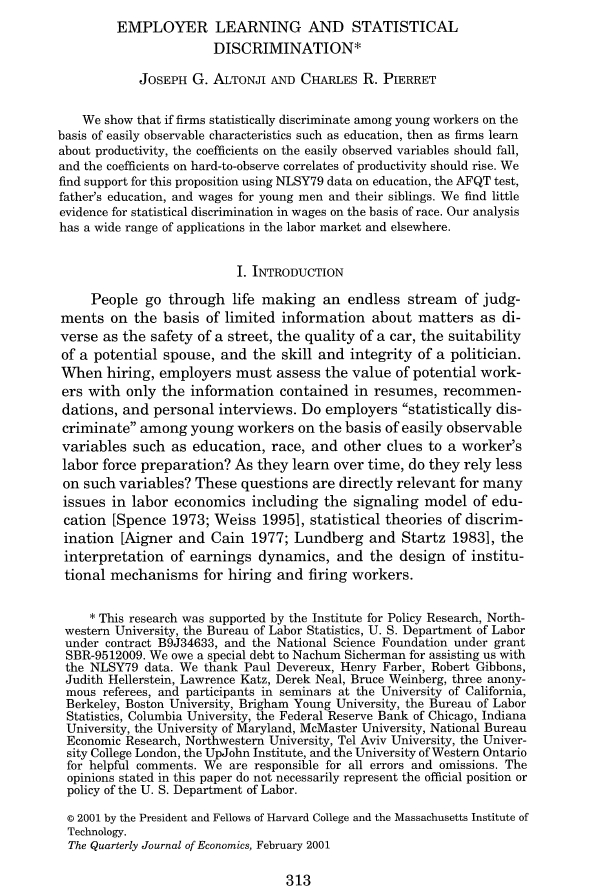
\includegraphics[width=0.44\textwidth, angle=-0.5]{Altonji_Pierret_2001_QJE_cover.jpg}
\end{frame}




\begin{frame}
IO papers that use learning models:
\bigskip\par
\begin{itemize}
\itemsep1.5em
\item Learning about experience goods (Erdem \& Keane 1996 MS)
\end{itemize}
\end{frame}

\begin{frame}
\centering
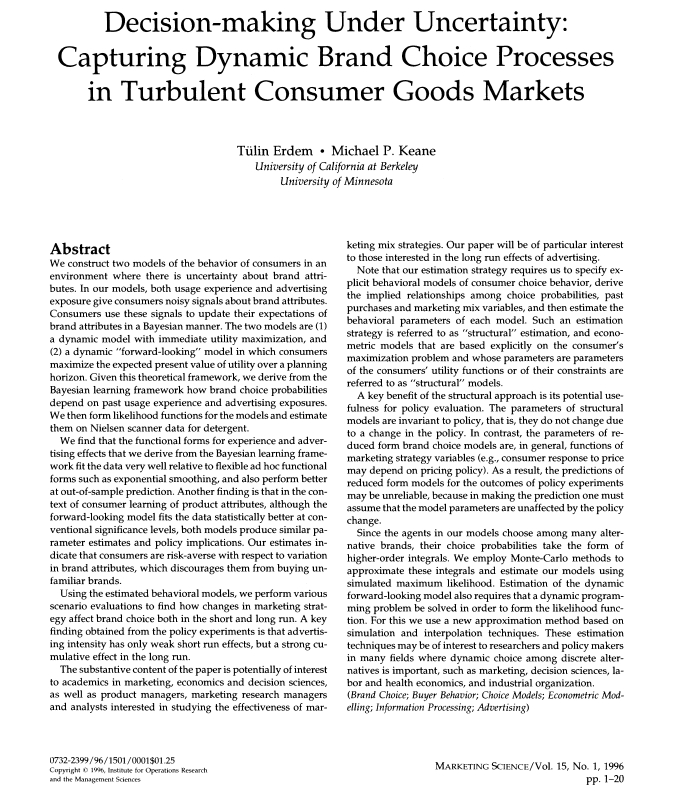
\includegraphics[width=0.52\textwidth]{Erdem_Keane_1996_MS_cover.jpg}
\end{frame}

\begin{frame}
IO papers that use learning models:
\bigskip\par
\begin{itemize}
\itemsep1.5em
\item Learning about experience goods (Erdem \& Keane 1996 MS; Ackerberg 2003 IER)
\end{itemize}
\end{frame}

\begin{frame}
\centering
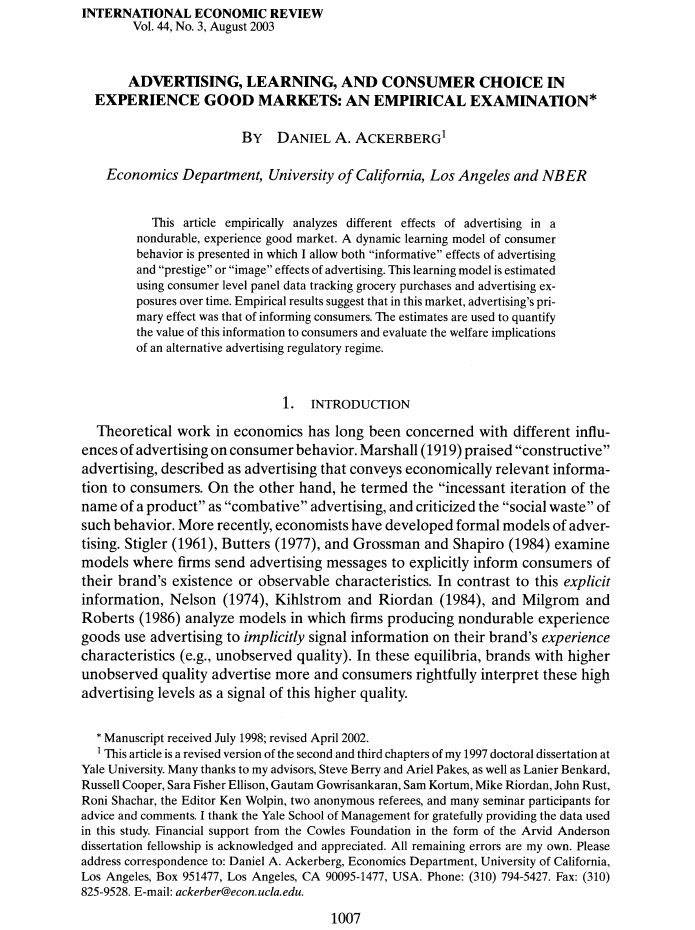
\includegraphics[width=0.45\textwidth]{Ackerberg_2003_IER_cover.jpg}
\end{frame}




\begin{frame}
Marriage \& family paper that uses learning models:
\bigskip\par
\begin{itemize}
\itemsep1.5em
\item Marriage match quality (Brien et al. 2006 IER)
\end{itemize}
\end{frame}

\begin{frame}
\centering
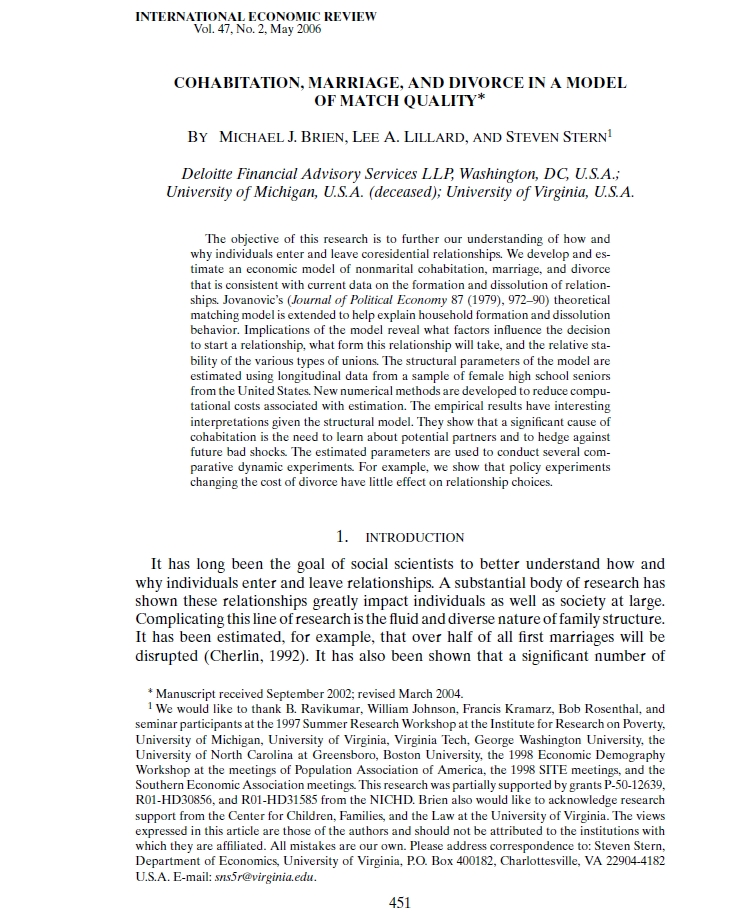
\includegraphics[width=0.52\textwidth]{Brien_et_al_2006_IER_cover.jpg}
\end{frame}

\end{document}
